
\documentclass[12pt]{article}
\usepackage{amssymb}
\usepackage{graphicx}
\usepackage{placeins}

\title{Development of Real-Time Systems}

\begin{document}

\maketitle

\section*{Assignment 4}

In this assignment we are going to use our previously learned skills in FreeRTOS and SimSo to schedule non-periodic jobs. First we will start off by setting up a set of periodic tasks in SimSo and then extend the schedule with a non-periodic job. We will compare difference schedulers here and argue for which one is better for different types of tasks. Then we will use FreeRTOS to implement non-periodic jobs in practice. With the previously learned skills in measuring time, we will measure the response time of non-periodic jobs and argue for or against a given schedule. 

\section{Simulation assignment}

Consider the tasks $T_{1}(3,\ 0.5)$, $T_{2}(4,\ 1.5,\ 3)$, $T_{3}(7,\ 1.0,\ 5)$ and the EDF scheduler. A sporadic job arrives at $t=50$ having the execution time of $10$ and a relative deadline of $30$. Create the sporadic task in SimSo by selecting: ”generate task set” and then list of act. Dates to the release time.

Use SimSo to schedule the task set and provide a report answering the following questions:

\begin{itemize}
\item \textbf{What is the minimum/maximum/average response time of all tasks?}

This data is shown on the task tab, which is presented on figure \ref{a_tasks_response_time}.

\begin{figure}[h]
\centering
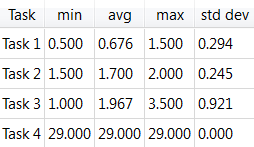
\includegraphics[scale=1]{figures/a_tasks_response_time}   
\caption{Task tab of results window in the first simulation.}
\label{a_tasks_response_time}
\end{figure}
\FloatBarrier

\item \textbf{Is any task missing the deadline? Which task? Where?}

No, all tasks meets the deadline as can be seen in the simulation log, which is presented on figure \ref{a_log}.

\begin{figure}[h]
\centering
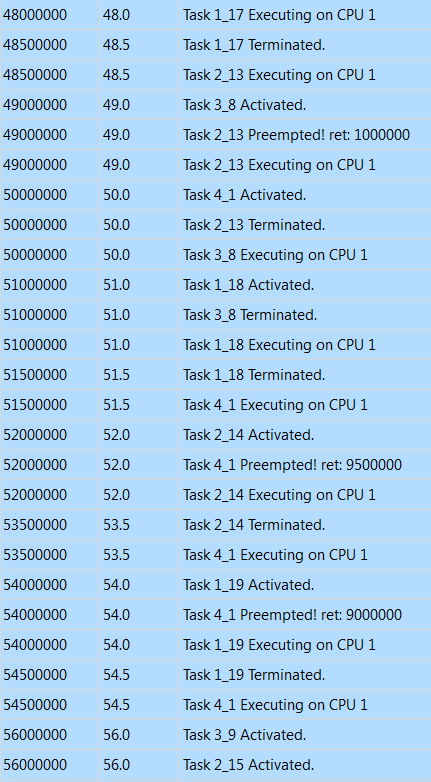
\includegraphics[scale=1]{figures/a_log}   
\caption{Log tab of results window in the first simulation.}
\label{a_log}
\end{figure}
\FloatBarrier

\item \textbf{Is the sporadic job meeting its deadline?}

Yes, it meets its deadline. In figure \ref{a_sporadic_gantt} it is shown how the sporadic job finish its execution at $t=79$ before the deadline which is at $t=80$.

\begin{figure}[h]
\centering
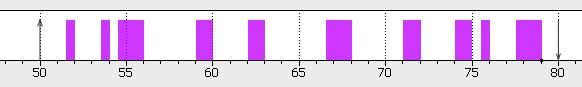
\includegraphics[scale=1]{figures/a_sporadic_gantt}   
\caption{Sporadic task Gantt diagram.}
\label{a_sporadic_gantt}
\end{figure}
\FloatBarrier

\item \textbf{What is the response time for the sporadic job?}

Like it was shown on figure \ref{a_tasks_response_time}, it has a response time of $29$.

\end{itemize}

Consider the tasks $T_{1}(3,\ 0.5)$, $T_{2}(4,\ 1.5,\ 3)$, $T_{3}(7,\ 1.0,\ 5)$ and the RM scheduler. A sporadic job arrives at $t=50$ having the execution time of $10$ and a relative deadline of $30$. Create the sporadic task in SimSo by selecting: ”generate task set” and then list of act. Dates to the release time.

Use SimSo to schedule the task set and provide a report answering the following questions:

\begin{itemize}
\item \textbf{What is the minimum/maximum/average response time of all tasks?}

This data is shown on the task tab, which is presented on figure \ref{b_tasks_response_time}.

\begin{figure}[h]
\centering
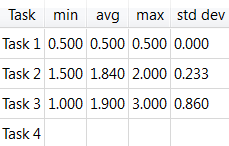
\includegraphics[scale=1]{figures/b_tasks_response_time}   
\caption{Task tab of results window in the second simulation.}
\label{b_tasks_response_time}
\end{figure}
\FloatBarrier

\item \textbf{Is any task missing the deadline? Which task? Where?}

Yes, Task 4, the sporadic task, miss its deadline. In figure \ref{b_log}, it can be seen that Task 4 aborts at time $80$ without finishing its execution.

\begin{figure}[h]
\centering
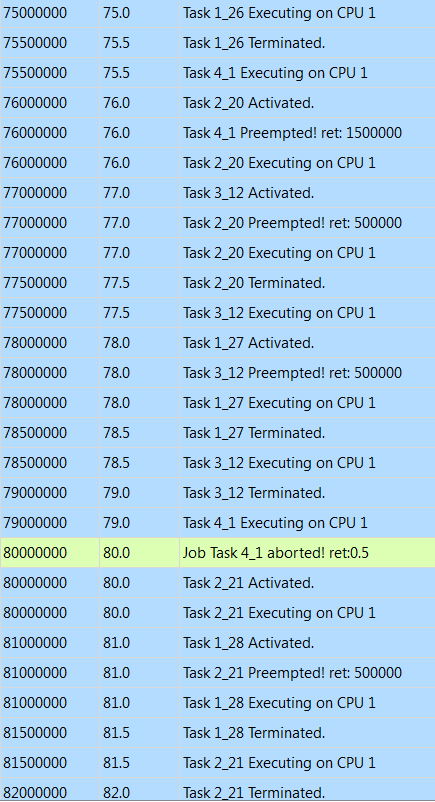
\includegraphics[scale=1]{figures/b_log}   
\caption{Log tab of results window in the second simulation.}
\label{b_log}
\end{figure}
\FloatBarrier

\item \textbf{Is the sporadic job meeting its deadline?}

No, it fails and aborts.

\item \textbf{What is the response time for the sporadic job?}

This can't be calculated since the sporadic job aborts its execution.

\item \textbf{Which scheduler is better is better in this example; EDF or RM?}

The best scheduler is EDF because it can provide feasibility to the system.

\end{itemize}


\section{Programming assignment}

The following questions should be solved with programming and the questions should be answered in a report.

\begin{itemize}
\item \textbf{Is the system fast enough to handle all aperiodic tasks? Why?}

No, aperiodic tasks tend to be blocked due to their low priority.

\item \textbf{If not, solve this problem without alter the functionality of any task}

The solution proposed is to elevate the priority from 2 to 4.

\item \textbf{What is the response time of the aperiodic task?}

The response time of the aperiodic task is about $2.08\ s$, like is shown on the program output on figure \ref{output}.

\item \textbf{Provide a screenshot of the running system}

\begin{figure}[h]
\centering
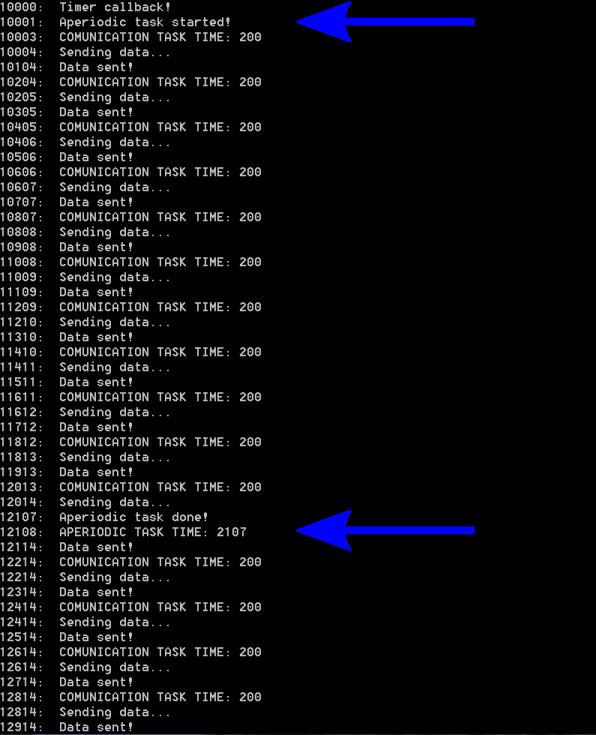
\includegraphics[scale=1]{figures/output}   
\caption{Screenshot of the running system.}
\label{output}
\end{figure}
\FloatBarrier

\end{itemize}
      
\end{document}